% Options for packages loaded elsewhere
\PassOptionsToPackage{unicode}{hyperref}
\PassOptionsToPackage{hyphens}{url}
%
\documentclass[
  man]{apa6}
\usepackage{amsmath,amssymb}
\usepackage{iftex}
\ifPDFTeX
  \usepackage[T1]{fontenc}
  \usepackage[utf8]{inputenc}
  \usepackage{textcomp} % provide euro and other symbols
\else % if luatex or xetex
  \usepackage{unicode-math} % this also loads fontspec
  \defaultfontfeatures{Scale=MatchLowercase}
  \defaultfontfeatures[\rmfamily]{Ligatures=TeX,Scale=1}
\fi
\usepackage{lmodern}
\ifPDFTeX\else
  % xetex/luatex font selection
\fi
% Use upquote if available, for straight quotes in verbatim environments
\IfFileExists{upquote.sty}{\usepackage{upquote}}{}
\IfFileExists{microtype.sty}{% use microtype if available
  \usepackage[]{microtype}
  \UseMicrotypeSet[protrusion]{basicmath} % disable protrusion for tt fonts
}{}
\makeatletter
\@ifundefined{KOMAClassName}{% if non-KOMA class
  \IfFileExists{parskip.sty}{%
    \usepackage{parskip}
  }{% else
    \setlength{\parindent}{0pt}
    \setlength{\parskip}{6pt plus 2pt minus 1pt}}
}{% if KOMA class
  \KOMAoptions{parskip=half}}
\makeatother
\usepackage{xcolor}
\usepackage{graphicx}
\makeatletter
\def\maxwidth{\ifdim\Gin@nat@width>\linewidth\linewidth\else\Gin@nat@width\fi}
\def\maxheight{\ifdim\Gin@nat@height>\textheight\textheight\else\Gin@nat@height\fi}
\makeatother
% Scale images if necessary, so that they will not overflow the page
% margins by default, and it is still possible to overwrite the defaults
% using explicit options in \includegraphics[width, height, ...]{}
\setkeys{Gin}{width=\maxwidth,height=\maxheight,keepaspectratio}
% Set default figure placement to htbp
\makeatletter
\def\fps@figure{htbp}
\makeatother
\setlength{\emergencystretch}{3em} % prevent overfull lines
\providecommand{\tightlist}{%
  \setlength{\itemsep}{0pt}\setlength{\parskip}{0pt}}
\setcounter{secnumdepth}{-\maxdimen} % remove section numbering
% Make \paragraph and \subparagraph free-standing
\makeatletter
\ifx\paragraph\undefined\else
  \let\oldparagraph\paragraph
  \renewcommand{\paragraph}{
    \@ifstar
      \xxxParagraphStar
      \xxxParagraphNoStar
  }
  \newcommand{\xxxParagraphStar}[1]{\oldparagraph*{#1}\mbox{}}
  \newcommand{\xxxParagraphNoStar}[1]{\oldparagraph{#1}\mbox{}}
\fi
\ifx\subparagraph\undefined\else
  \let\oldsubparagraph\subparagraph
  \renewcommand{\subparagraph}{
    \@ifstar
      \xxxSubParagraphStar
      \xxxSubParagraphNoStar
  }
  \newcommand{\xxxSubParagraphStar}[1]{\oldsubparagraph*{#1}\mbox{}}
  \newcommand{\xxxSubParagraphNoStar}[1]{\oldsubparagraph{#1}\mbox{}}
\fi
\makeatother
% definitions for citeproc citations
\NewDocumentCommand\citeproctext{}{}
\NewDocumentCommand\citeproc{mm}{%
  \begingroup\def\citeproctext{#2}\cite{#1}\endgroup}
\makeatletter
 % allow citations to break across lines
 \let\@cite@ofmt\@firstofone
 % avoid brackets around text for \cite:
 \def\@biblabel#1{}
 \def\@cite#1#2{{#1\if@tempswa , #2\fi}}
\makeatother
\newlength{\cslhangindent}
\setlength{\cslhangindent}{1.5em}
\newlength{\csllabelwidth}
\setlength{\csllabelwidth}{3em}
\newenvironment{CSLReferences}[2] % #1 hanging-indent, #2 entry-spacing
 {\begin{list}{}{%
  \setlength{\itemindent}{0pt}
  \setlength{\leftmargin}{0pt}
  \setlength{\parsep}{0pt}
  % turn on hanging indent if param 1 is 1
  \ifodd #1
   \setlength{\leftmargin}{\cslhangindent}
   \setlength{\itemindent}{-1\cslhangindent}
  \fi
  % set entry spacing
  \setlength{\itemsep}{#2\baselineskip}}}
 {\end{list}}
\usepackage{calc}
\newcommand{\CSLBlock}[1]{\hfill\break\parbox[t]{\linewidth}{\strut\ignorespaces#1\strut}}
\newcommand{\CSLLeftMargin}[1]{\parbox[t]{\csllabelwidth}{\strut#1\strut}}
\newcommand{\CSLRightInline}[1]{\parbox[t]{\linewidth - \csllabelwidth}{\strut#1\strut}}
\newcommand{\CSLIndent}[1]{\hspace{\cslhangindent}#1}
\ifLuaTeX
\usepackage[bidi=basic]{babel}
\else
\usepackage[bidi=default]{babel}
\fi
\babelprovide[main,import]{english}
% get rid of language-specific shorthands (see #6817):
\let\LanguageShortHands\languageshorthands
\def\languageshorthands#1{}
% Manuscript styling
\usepackage{upgreek}
\captionsetup{font=singlespacing,justification=justified}

% Table formatting
\usepackage{longtable}
\usepackage{lscape}
% \usepackage[counterclockwise]{rotating}   % Landscape page setup for large tables
\usepackage{multirow}		% Table styling
\usepackage{tabularx}		% Control Column width
\usepackage[flushleft]{threeparttable}	% Allows for three part tables with a specified notes section
\usepackage{threeparttablex}            % Lets threeparttable work with longtable

% Create new environments so endfloat can handle them
% \newenvironment{ltable}
%   {\begin{landscape}\centering\begin{threeparttable}}
%   {\end{threeparttable}\end{landscape}}
\newenvironment{lltable}{\begin{landscape}\centering\begin{ThreePartTable}}{\end{ThreePartTable}\end{landscape}}

% Enables adjusting longtable caption width to table width
% Solution found at http://golatex.de/longtable-mit-caption-so-breit-wie-die-tabelle-t15767.html
\makeatletter
\newcommand\LastLTentrywidth{1em}
\newlength\longtablewidth
\setlength{\longtablewidth}{1in}
\newcommand{\getlongtablewidth}{\begingroup \ifcsname LT@\roman{LT@tables}\endcsname \global\longtablewidth=0pt \renewcommand{\LT@entry}[2]{\global\advance\longtablewidth by ##2\relax\gdef\LastLTentrywidth{##2}}\@nameuse{LT@\roman{LT@tables}} \fi \endgroup}

% \setlength{\parindent}{0.5in}
% \setlength{\parskip}{0pt plus 0pt minus 0pt}

% Overwrite redefinition of paragraph and subparagraph by the default LaTeX template
% See https://github.com/crsh/papaja/issues/292
\makeatletter
\renewcommand{\paragraph}{\@startsection{paragraph}{4}{\parindent}%
  {0\baselineskip \@plus 0.2ex \@minus 0.2ex}%
  {-1em}%
  {\normalfont\normalsize\bfseries\itshape\typesectitle}}

\renewcommand{\subparagraph}[1]{\@startsection{subparagraph}{5}{1em}%
  {0\baselineskip \@plus 0.2ex \@minus 0.2ex}%
  {-\z@\relax}%
  {\normalfont\normalsize\itshape\hspace{\parindent}{#1}\textit{\addperi}}{\relax}}
\makeatother

\makeatletter
\usepackage{etoolbox}
\patchcmd{\maketitle}
  {\section{\normalfont\normalsize\abstractname}}
  {\section*{\normalfont\normalsize\abstractname}}
  {}{\typeout{Failed to patch abstract.}}
\patchcmd{\maketitle}
  {\section{\protect\normalfont{\@title}}}
  {\section*{\protect\normalfont{\@title}}}
  {}{\typeout{Failed to patch title.}}
\makeatother

\usepackage{xpatch}
\makeatletter
\xapptocmd\appendix
  {\xapptocmd\section
    {\addcontentsline{toc}{section}{\appendixname\ifoneappendix\else~\theappendix\fi: #1}}
    {}{\InnerPatchFailed}%
  }
{}{\PatchFailed}
\makeatother
\keywords{Reproducibility, R, Teaching, Demonstration\newline\indent Word count: X}
\DeclareDelayedFloatFlavor{ThreePartTable}{table}
\DeclareDelayedFloatFlavor{lltable}{table}
\DeclareDelayedFloatFlavor*{longtable}{table}
\makeatletter
\renewcommand{\efloat@iwrite}[1]{\immediate\expandafter\protected@write\csname efloat@post#1\endcsname{}}
\makeatother
\usepackage{lineno}

\linenumbers
\usepackage{csquotes}
\ifLuaTeX
  \usepackage{selnolig}  % disable illegal ligatures
\fi
\usepackage{bookmark}
\IfFileExists{xurl.sty}{\usepackage{xurl}}{} % add URL line breaks if available
\urlstyle{same}
\hypersetup{
  pdftitle={Lecture 12: Preparing journal artical with papaja},
  pdfauthor={Hu Chuan-Peng1 \& All Students1,2},
  pdflang={en-EN},
  pdfkeywords={Reproducibility, R, Teaching, Demonstration},
  hidelinks,
  pdfcreator={LaTeX via pandoc}}

\title{Lecture 12: Preparing journal artical with \emph{papaja}}
\author{Hu Chuan-Peng\textsuperscript{1} \& All Students\textsuperscript{1,2}}
\date{}


\shorttitle{papaja}

\authornote{

Add complete departmental affiliations for each author here. Each new line herein must be indented, like this line.

Author Note: This is for demonstration only.

The authors made the following contributions. Hu Chuan-Peng: Conceptualization, Writing - Original Draft Preparation, Supervision; All Students: Writing - Original Draft Preparation, Writing - Review \& Editing.

Correspondence concerning this article should be addressed to Hu Chuan-Peng, \#122 Ninghai Rd, Gulou District, Nanjing. E-mail: \href{mailto:hcp4715@hotmail.com}{\nolinkurl{hcp4715@hotmail.com}}

}

\affiliation{\vspace{0.5cm}\textsuperscript{1} Nanjing Normal Unviersity\\\textsuperscript{2} Collaborators' Affiliations}

\abstract{%
Psychological science has encountered a serious replication crisis.

To make self-correction of the field, researchers actively reform the current practices and increase the opennes, transparency, and reproducibility of studies in the field. Using R language for data analyses is recommended by many. With increasingly emphases on computational reproduciblity, \emph{papaja} was developed to combine data analysis and manuscript preparation.

The current chapter aims to demonstrate how to use \emph{papaja}.

We will introduce the package and key elements of the it.

After the lecture, we expected students able to create an example APA manuscript using open data or examplary data we had provided at the beginning of the class.

This demo and practice will further enhance the student's experience in computational reproducibility.

By spreading the ideas of reproducbility and teaching papaja, this class will increase the computational reprodcubility.
}



\begin{document}
\maketitle

R language has been widely used in psychological science and social science in general. However, for most students with a background of psychology, learning R is not easy.

In the past decade, an increasingly number of psychological researchers had switched from SPSS to R. The most common suggestions from those who successfully adopted R is: learning by doing.

To fully integrate R in the life-cycle of psychological research, using R for preparing journal article is necessary.

Fortunately, we now have \emph{papaja} (Aust \& Barth, 2024), which enable us to prepare journal article that formatted as required by APA.

Below we will demonstrate how to use \emph{papaja} to generate an APA formatted PDF. Note that we will use the data from perceptual matching task, which was from (Hu, Lan, Macrae, \& Sui, 2020). The data analysis for this dataset has been showed in previous classes.

Here we will try to reproduce what has been reported in Hu et al. (2020). Thus, we adopted the code from: \url{https://github.com/hcp4715/moralSelf_ddm}.

\section{Methods}\label{methods}

We report how we determined our sample size, all data exclusions (if any), all manipulations, and all measures in the study.

\subsection{Participants}\label{participants}

The sample size of the study was determined in a dynamic way (Schoenbrodt, Wagenmakers, Zehetleitner, \& Perugini, 2017). Specifically, we kept collecting data and analyzing the strength of evidence for the critical hypothesis, including the interaction between Self-Relevance × Valence on RT data and two Bayes factor paired \emph{t}-tests (good-self vs.~bad-self, good-self vs.~good-other). We stopped recruiting new participants when both paired \emph{t}-tests reached \(BF_{10} \le 0.1\) or \(BF_{10} \ge 10\). Participants who were already recruited at that moment continued to complete the experiment. See \url{https://osf.io/w6hrj/} for the change of Bayes factor during the data collection. In total, 44 college students (25 females, age: 20.91 \(\pm\) 2.58) were recruited. Two participants were excluded from data analysis because of procedural failures, leaving 42 participants (24 females, age: 20.71 \(\pm\) 2.38).

\subsection{Material and Procedure}\label{material-and-procedure}

The data was collected using the same settings as described in the pilot study, with several differences:

\begin{itemize}
\tightlist
\item
  In the shape-categorization task, the shapes were presented for 100 ms, instead of 200 ms in the pilot experiment, and feedback was Chinese character `Correct' or `Incorrect', instead of happy or sad symbolic faces.
\item
  There were only two different types of blocks in the categorization task in the confirmatory study because the importance judgments resulted in unbalanced trials between participants.
\item
  There were more trials per condition: 72 experimental trials for the matching task.
\item
  The questionnaires were different from the pilot study.
\end{itemize}

\subsection{Data analysis}\label{data-analysis}

We used R (Version 4.3.3; R Core Team, 2024) and the R-packages \emph{afex} (Version 1.4.1; Singmann, Bolker, Westfall, Aust, \& Ben-Shachar, 2024), \emph{dplyr} (Version 1.1.4; Wickham, François, Henry, Müller, \& Vaughan, 2023), \emph{emmeans} (Version 1.10.6; Lenth, 2024), \emph{ggplot2} (Version 3.5.1; Wickham, 2016), \emph{patchwork} (Version 1.3.0; Pedersen, 2024) and \emph{tidyr} (Version 1.3.1; Wickham, Vaughan, \& Girlich, 2024) for all our analyses. The results from Frequentist hypothesis testing (i.e., ANOVA and \emph{t}-tests) will be reported below.

\section{Results}\label{results}

\begin{figure}
\centering
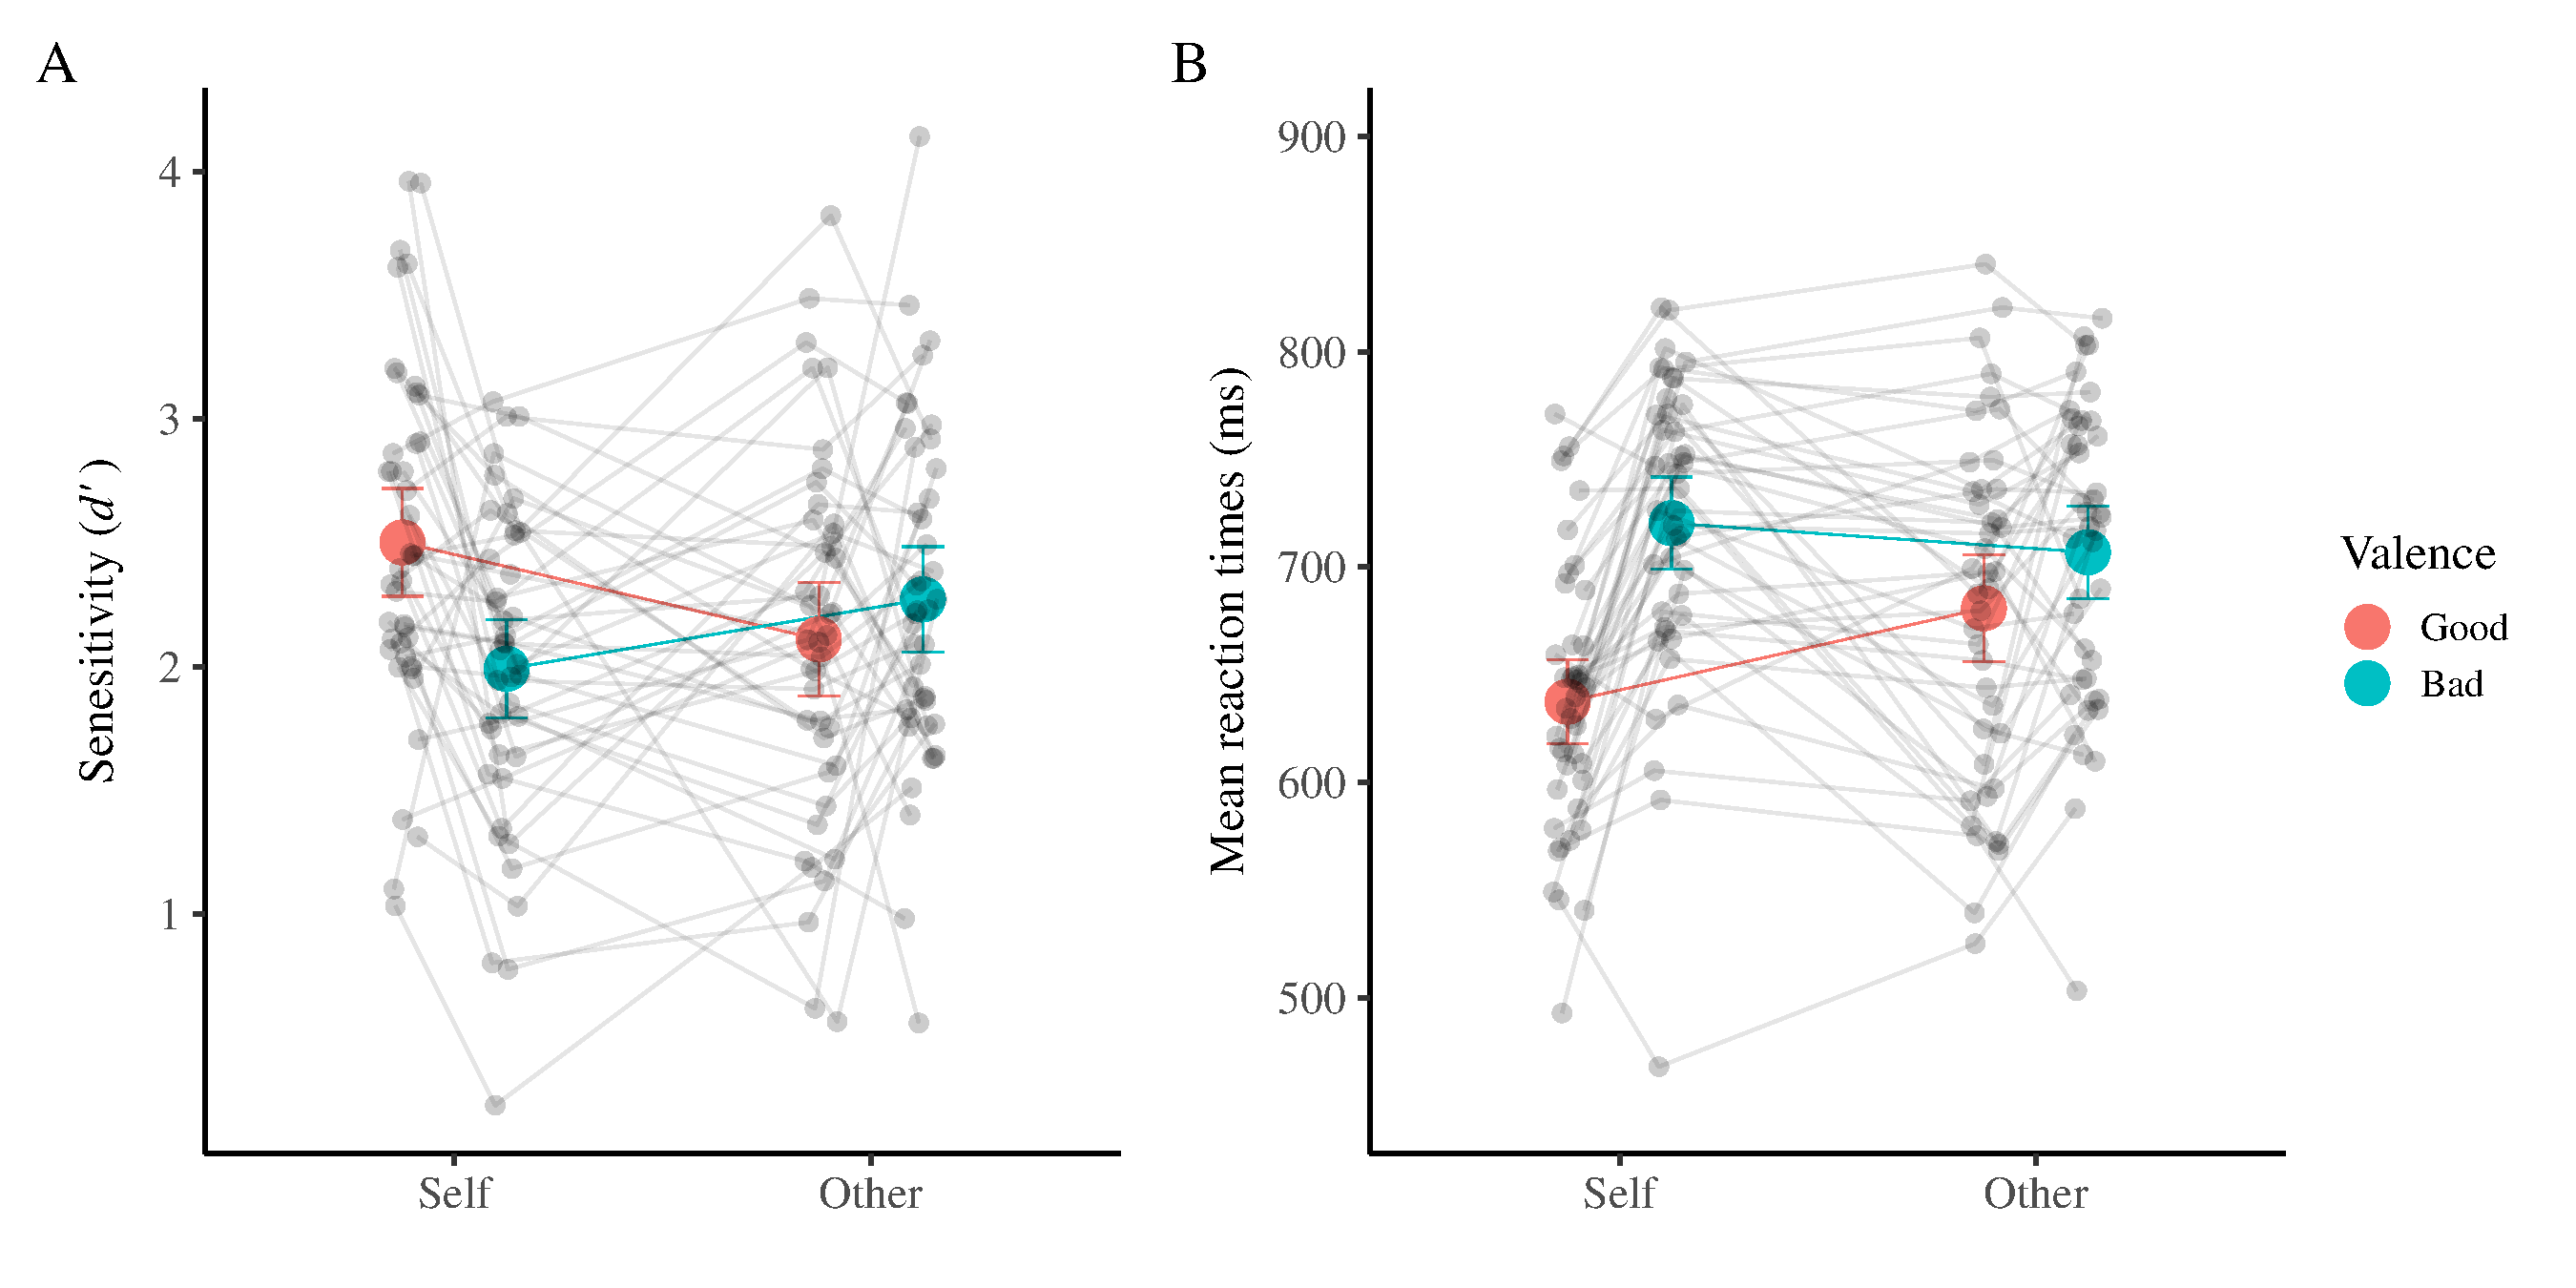
\includegraphics{chapter_12_pt2_papaja_files/figure-latex/plot1-1.pdf}
\caption{\label{fig:plot1}Interaction between identity and valence for (A) sensitivity and (B) reaction times.}
\end{figure}

\subsection{\texorpdfstring{Sensitivity (\emph{d'})}{Sensitivity (d')}}\label{sensitivity-d}

A two-way repeated-measure ANOVA revealed a significant interaction between Identity and Valence. \emph{F}(1, 41) = 12.06, \emph{p} = 0.0012. We conducted follow-up simple main effect analyses. When the shapes were self-referential, \emph{d'} was significantly larger for moral condition (2.5 \(\pm\) 0.11) than for immoral condition (1.99 \(\pm\) 0.1), \emph{t}(41) = 4.29, \emph{p} \textless{} 0.001. However, this was no clear evidence that moral condition (2.11 \(\pm\) 0.116) and immoral condition (2.27 \(\pm\) 0.107) were not significantly different when the shapes are other-referential (see figure \ref{fig:plot1}).

\subsection{Reaction times}\label{reaction-times}

{[}Please finish this part{]}

\section{Discussion}\label{discussion}

In this demonstration, we examplified how to use \emph{papaja} to prepare an APA style manuscript. We highlighted the following details:

\begin{itemize}
\tightlist
\item
  Installation and start a manuscript from the template.
\item
  YAML front
\item
  Mathematical notations
\item
  Citation
\item
  Insert results from code block
\item
  Plot
\end{itemize}

\newpage

\section{References}\label{references}

\phantomsection\label{refs}
\begin{CSLReferences}{1}{0}
\bibitem[\citeproctext]{ref-R-papaja}
Aust, F., \& Barth, M. (2024). \emph{{papaja}: {Prepare} reproducible {APA} journal articles with {R Markdown}}. \url{https://doi.org/10.32614/CRAN.package.papaja}

\bibitem[\citeproctext]{ref-Hu_2020}
Hu, C.-P., Lan, Y., Macrae, C. N., \& Sui, J. (2020). Good {Me} {Bad} {Me}: {Does} {Valence} {Influence} {Self}-{Prioritization} {During} {Perceptual} {Decision}-{Making}? \emph{Collabra-Psychology}, \emph{6}(1), 20. \url{https://doi.org/10.1525/collabra.301}

\bibitem[\citeproctext]{ref-R-emmeans}
Lenth, R. V. (2024). \emph{Emmeans: Estimated marginal means, aka least-squares means}. Retrieved from \url{https://CRAN.R-project.org/package=emmeans}

\bibitem[\citeproctext]{ref-R-patchwork}
Pedersen, T. L. (2024). \emph{Patchwork: The composer of plots}. Retrieved from \url{https://CRAN.R-project.org/package=patchwork}

\bibitem[\citeproctext]{ref-R-base}
R Core Team. (2024). \emph{R: A language and environment for statistical computing}. Vienna, Austria: R Foundation for Statistical Computing. Retrieved from \url{https://www.R-project.org/}

\bibitem[\citeproctext]{ref-schoenbrodt_sequential_2017}
Schoenbrodt, F. D., Wagenmakers, E.-J., Zehetleitner, M., \& Perugini, M. (2017). Sequential hypothesis testing with {Bayes} factors: {Efficiently} testing mean differences. \emph{Psychological Methods}, \emph{22}(2), 322--339. \url{https://doi.org/10.1037/met0000061}

\bibitem[\citeproctext]{ref-R-afex}
Singmann, H., Bolker, B., Westfall, J., Aust, F., \& Ben-Shachar, M. S. (2024). \emph{Afex: Analysis of factorial experiments}. Retrieved from \url{https://CRAN.R-project.org/package=afex}

\bibitem[\citeproctext]{ref-R-ggplot2}
Wickham, H. (2016). \emph{ggplot2: Elegant graphics for data analysis}. Springer-Verlag New York. Retrieved from \url{https://ggplot2.tidyverse.org}

\bibitem[\citeproctext]{ref-R-dplyr}
Wickham, H., François, R., Henry, L., Müller, K., \& Vaughan, D. (2023). \emph{Dplyr: A grammar of data manipulation}. Retrieved from \url{https://CRAN.R-project.org/package=dplyr}

\bibitem[\citeproctext]{ref-R-tidyr}
Wickham, H., Vaughan, D., \& Girlich, M. (2024). \emph{Tidyr: Tidy messy data}. Retrieved from \url{https://CRAN.R-project.org/package=tidyr}

\end{CSLReferences}


\end{document}
